
\documentclass[11pt]{article}\usepackage[]{graphicx}\usepackage[]{color}
%% maxwidth is the original width if it is less than linewidth
%% otherwise use linewidth (to make sure the graphics do not exceed the margin)
\makeatletter
\def\maxwidth{ %
  \ifdim\Gin@nat@width>\linewidth
    \linewidth
  \else
    \Gin@nat@width
  \fi
}
\makeatother

\definecolor{fgcolor}{rgb}{0.345, 0.345, 0.345}
\newcommand{\hlnum}[1]{\textcolor[rgb]{0.686,0.059,0.569}{#1}}%
\newcommand{\hlstr}[1]{\textcolor[rgb]{0.192,0.494,0.8}{#1}}%
\newcommand{\hlcom}[1]{\textcolor[rgb]{0.678,0.584,0.686}{\textit{#1}}}%
\newcommand{\hlopt}[1]{\textcolor[rgb]{0,0,0}{#1}}%
\newcommand{\hlstd}[1]{\textcolor[rgb]{0.345,0.345,0.345}{#1}}%
\newcommand{\hlkwa}[1]{\textcolor[rgb]{0.161,0.373,0.58}{\textbf{#1}}}%
\newcommand{\hlkwb}[1]{\textcolor[rgb]{0.69,0.353,0.396}{#1}}%
\newcommand{\hlkwc}[1]{\textcolor[rgb]{0.333,0.667,0.333}{#1}}%
\newcommand{\hlkwd}[1]{\textcolor[rgb]{0.737,0.353,0.396}{\textbf{#1}}}%

\usepackage{framed}
\makeatletter
\newenvironment{kframe}{%
 \def\at@end@of@kframe{}%
 \ifinner\ifhmode%
  \def\at@end@of@kframe{\end{minipage}}%
  \begin{minipage}{\columnwidth}%
 \fi\fi%
 \def\FrameCommand##1{\hskip\@totalleftmargin \hskip-\fboxsep
 \colorbox{shadecolor}{##1}\hskip-\fboxsep
     % There is no \\@totalrightmargin, so:
     \hskip-\linewidth \hskip-\@totalleftmargin \hskip\columnwidth}%
 \MakeFramed {\advance\hsize-\width
   \@totalleftmargin\z@ \linewidth\hsize
   \@setminipage}}%
 {\par\unskip\endMakeFramed%
 \at@end@of@kframe}
\makeatother

\definecolor{shadecolor}{rgb}{.97, .97, .97}
\definecolor{messagecolor}{rgb}{0, 0, 0}
\definecolor{warningcolor}{rgb}{1, 0, 1}
\definecolor{errorcolor}{rgb}{1, 0, 0}
\newenvironment{knitrout}{}{} % an empty environment to be redefined in TeX

\usepackage{alltt}

% margins, size, formatting

\oddsidemargin=0in
\evensidemargin=0in
\topmargin=0in
\textwidth=6.5in
\textheight=9.5in
\parindent = 0 in
%\pagestyle{plain}
\pagestyle{plain}

\usepackage{amsmath,amssymb,amsthm, amsfonts}
\usepackage{array}
\usepackage{fancyhdr}
%\pagestyle{plain}
\pagestyle{fancy}
\usepackage[bottom=0.5in]{geometry}
%\usepackage{listings}
%\usepackage{inconsolata}

\lhead{\textbf{Group 3: Data Analysis\\ Spring 2014}}
\rhead{\textbf{Nick Cummings, Liza Nicoll \\ Emily Ramos and Yiding Zhang}}
\cfoot{}
\IfFileExists{upquote.sty}{\usepackage{upquote}}{}

\begin{document}

\section{Introduction} %Emily

The dataset we will be using for our group analysis is ``Exploring Relationships in Body Dimensions". This dataset contains information on 21 body dimension measurements (including skeletal measurements and girth measurments) as well as age, weight, height and gender from 507 physically active men and women within the normal weight range. Most of these individuals are in their 20s and 30s. The initial reason the data was collected was to determine how well weight could be predicted between body build, weight, and girths. \\ 

This analysis will include our group analysis: summary of the dataset, our hypothesis, the base model we will be using, applications of the data and model, and our individual analyses: regression trees, model selection, resampling inference, bootstrapping, logistic regression and Ada-boosting.

%------------------------------------------------
\section{Group Analysis} 





%------------------------------------------------

\subsection{Summary of the Dataset}

%-------------------------------------------------
\\

\textbf{Variables in the Dataset}\\ %Emily

There are a total of 25 variables.\\

Skeletal measurements include: biacromial diameter, pelvic breadth, bitrochanteric diameter, chest depth, chest diameter, elbow diameter, wrist diameter, knee and ankle diameter. Note that elbow, wrist, knee and ankle measurements are the sum of the two ankle diameters.\\

Girth measurements include: shoulder, chest, waist, navel, hip, thigh, flexed bicep, extended forearm, knee, calf maximum, ankle minimum and wrist minimum. Note, for thigh, bicep, forearm, knee, calf, ankle and wrist girth measurments the average of both body parts was taken.\\

Other measurements include: age, weight, height and gender (male= 1 and femal = 0).\\

%------------------------------------------------

\newpage

\textbf{Weight}\\ %Liza
   
Weight was measured for 507 physically active individuals - 247 men and 260 women. The distribution ranged from 42 kilograms to 116.4 kilograms. The mean weight and quartiles was signifigantly higher for men than women. We observe several outliers in the upper end of the range for both men and women. This may be due to the fact that the population sampled included a number of highly physicaly fit individuals with higher than average muscle mass.

\begin{knitrout}
\definecolor{shadecolor}{rgb}{0.969, 0.969, 0.969}\color{fgcolor}
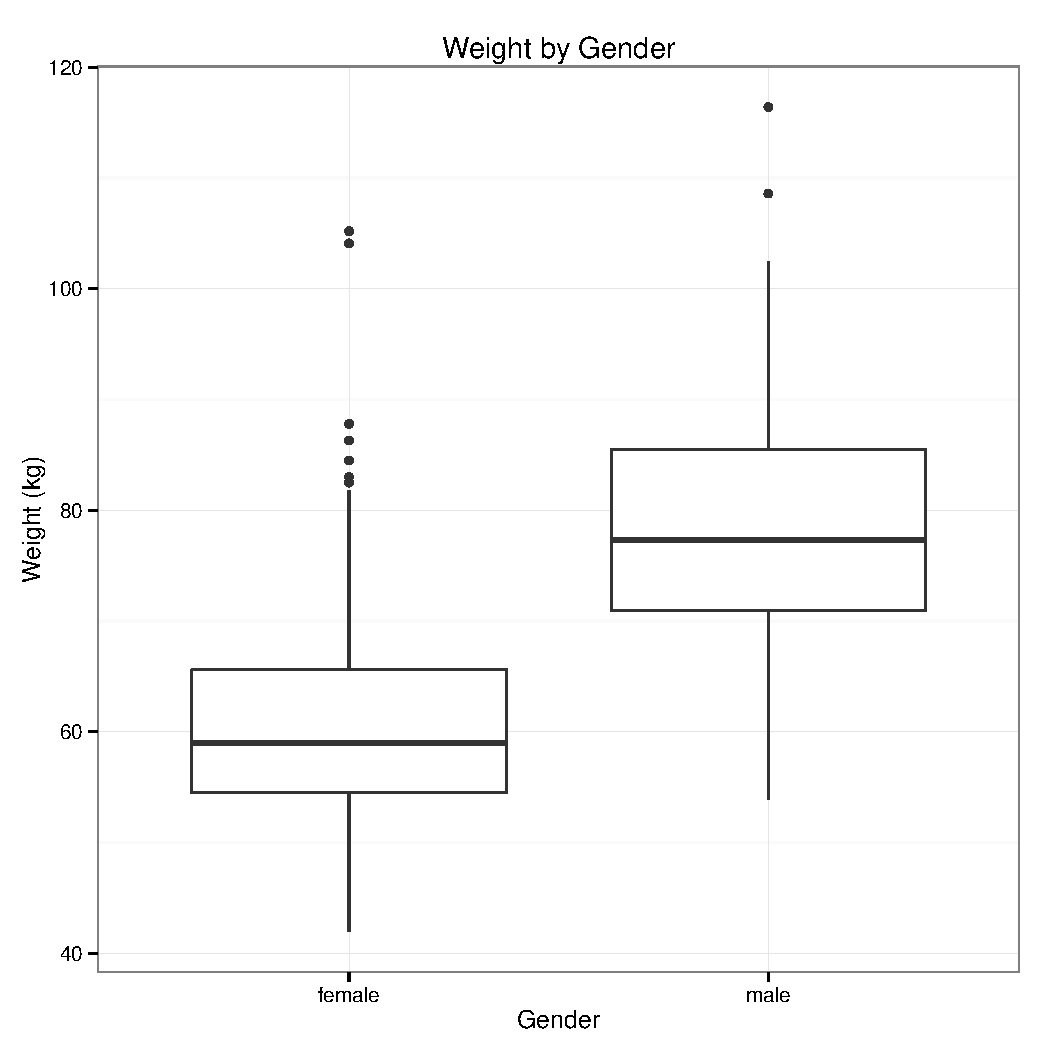
\includegraphics[width=\maxwidth]{figure/weight_plot} 

\end{knitrout}


%------------------------------------------------

\newpage

\textbf{Bitrochanteric Diameter and Hip Girth}\\ %Liza
 
Bitrochanteric diameter is the distance between the outer points of the hips and hip girth is the circumference of the hip area measured at the level of the bitrochanteric diameter. The density distributions for both measures are normally distributed (though hip girth is skewed slightly right) and very similar in distribution for both men and women. A scatter plot of hip girth vs. weight suggests that weight increases linerally with increase in hip girth.

\begin{knitrout}
\definecolor{shadecolor}{rgb}{0.969, 0.969, 0.969}\color{fgcolor}
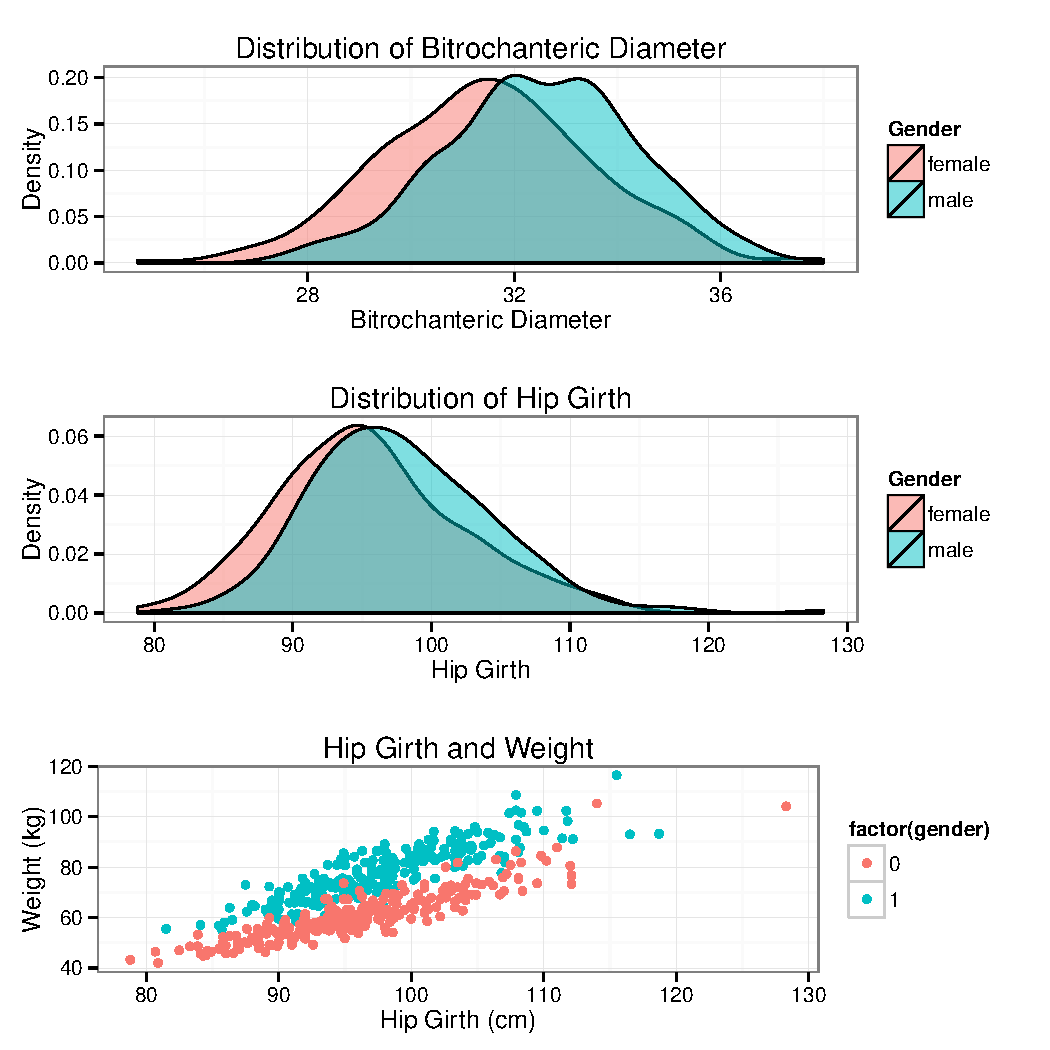
\includegraphics[width=\maxwidth]{figure/hip_plots} 

\end{knitrout}



\begin{knitrout}
\definecolor{shadecolor}{rgb}{0.969, 0.969, 0.969}\color{fgcolor}
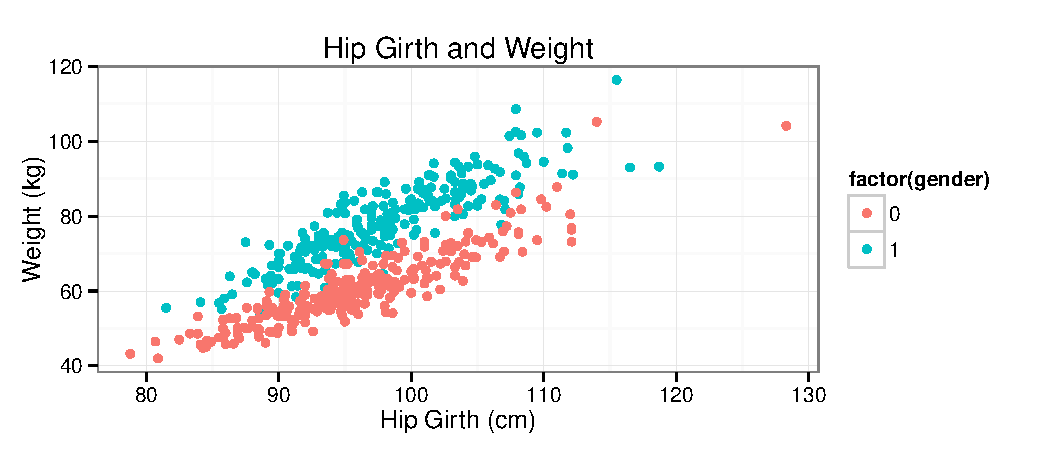
\includegraphics[width=\maxwidth]{figure/hipgirth_plot} 

\end{knitrout}


%------------------------------------------------

\newpage

\textbf{Chest and Shoulder}\\ %Liza
   
Chest girth was measured at the nipple line in males and just above breast tissue in females at mid-expiration and shoulder girth was measured over deltoid muscles in both males and females. The density distributions for the two variables are quite similar. Women have narrower, though slightly skeewed, distribution with a much lower mean than that of the men. The scatterplots are also similar in that the regression lines for men and women are nearly identical, indicating that weight increases linearly with increase in shoulder girth, independant of gender.

\begin{knitrout}
\definecolor{shadecolor}{rgb}{0.969, 0.969, 0.969}\color{fgcolor}
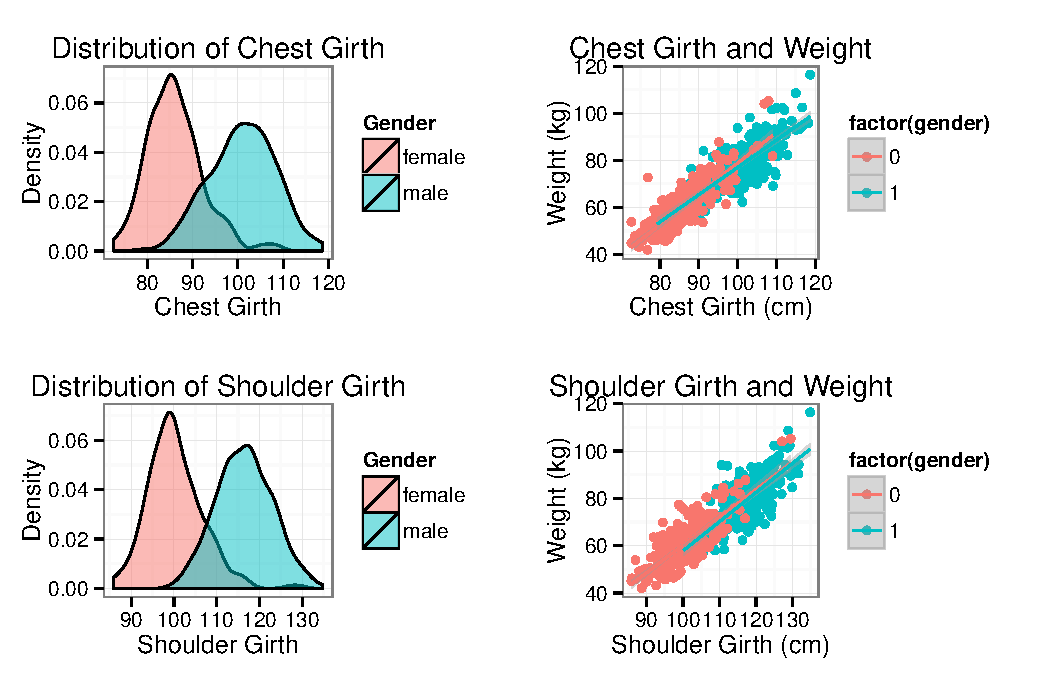
\includegraphics[width=\maxwidth]{figure/chest_plots} 

\end{knitrout}


%------------------------------------------------

\newpage

\textbf{Wrist and Navel}\\ %Liza
   
Wrist minimum girth is an average of right and left girths and navel (or abdominal) girth was measured at umbilicus and the iliac crest, using the iliac crest as a landmark. Wrist girth is bimodally distributed, but when divided into male and female, the distributions are normal with some outliers at the high end of the range for females. The distributions for navel girth is normal and remarkably similar for males and females. The scatterplot of navel girth against weight shows a linear relationship with weight increasing with increased naval girth.

\begin{knitrout}
\definecolor{shadecolor}{rgb}{0.969, 0.969, 0.969}\color{fgcolor}
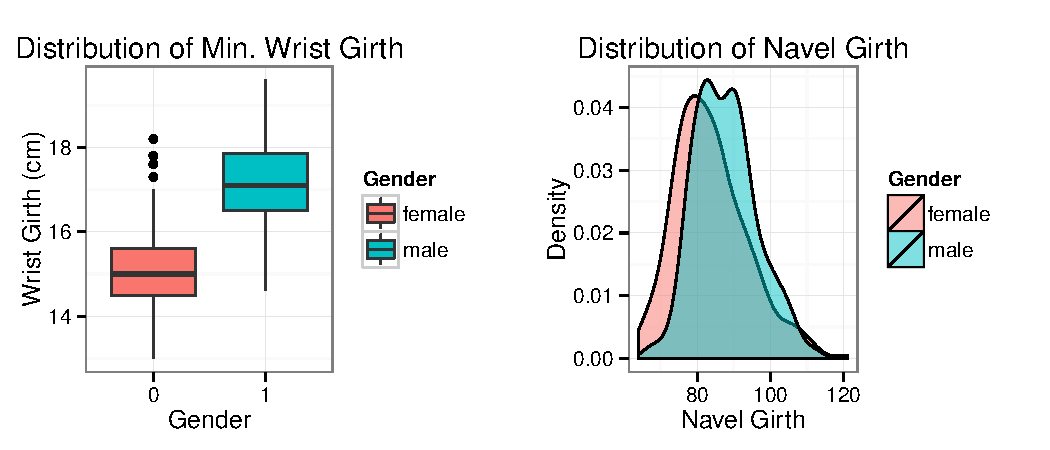
\includegraphics[width=\maxwidth]{figure/navel_plots} 

\end{knitrout}


\begin{knitrout}
\definecolor{shadecolor}{rgb}{0.969, 0.969, 0.969}\color{fgcolor}
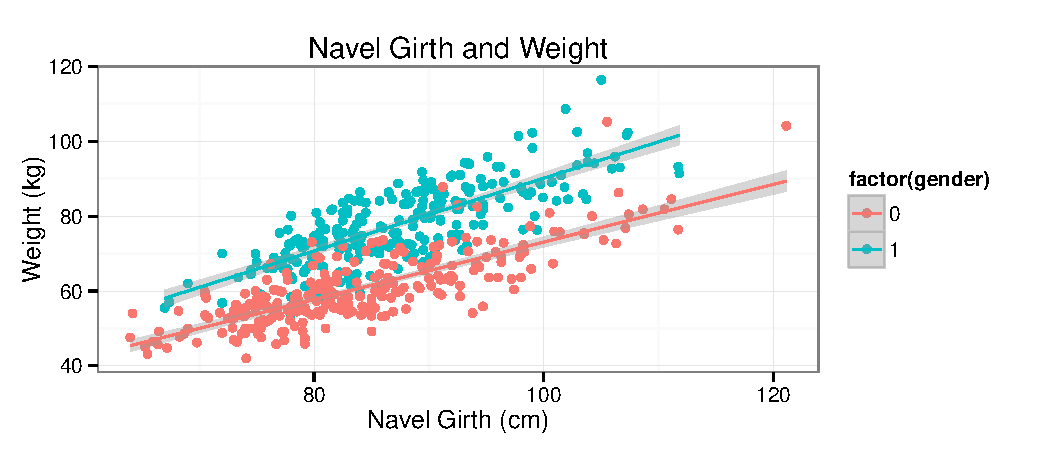
\includegraphics[width=\maxwidth]{figure/navelgirth_plot} 

\end{knitrout}


\newpage

\textbf{Age and Weight}\\ %Yiding

Since our dataset contains information on \textit{mostly} individuals in their 20s and 30s, we should check how age and weight intereact in our data before conducting analysis on weight. The mean age is 30, the youngest subject is 18 and the oldes subject is 67. The first plot shows that age is unevenly distributed, i.e left skewed. Most of the subjects are physically active young individuals. Since we have this skewness of data, we seperate the data into two subsets- young and middle age to see how weight interacts in these subsets. The weight of young and middle age groups are generally normally distributed and are remarkably similar. This shows that, although our ages are skewed, we can apply this analysis to physically active individuals of all ages.

\begin{knitrout}
\definecolor{shadecolor}{rgb}{0.969, 0.969, 0.969}\color{fgcolor}
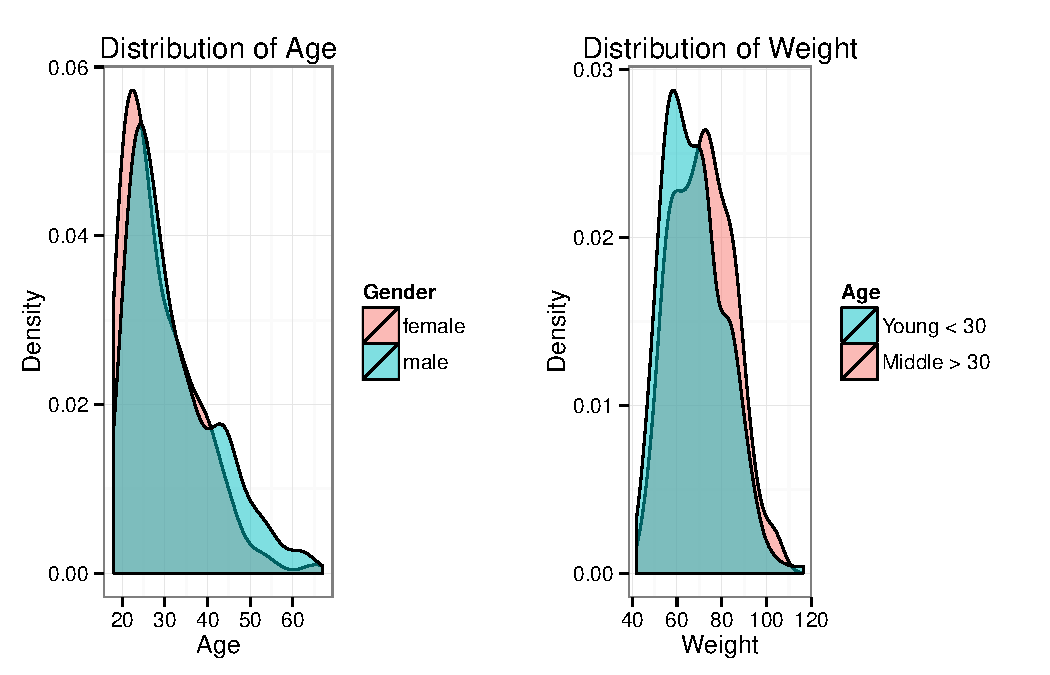
\includegraphics[width=\maxwidth]{figure/unnamed-chunk-1} 

\end{knitrout}



%------------------------------------------------

\subsection{Initial Multiple Linear Regression Model} 

%------------------------------------------------

\subsubsection{Hypothesises}%Yiding

%------------------------------------------------

\textbf{Weight}\\ 
In two ways one can get a plausible model: statistical analysis and experience. Upon initial exploration, we notice that several variables have high $p$-values, such as navel girth and flexed bicep. From a statistical perspective, these variables may be considerated as non-significant variables; however, in the paper, the author use the initial model with a adjusted $R^2 = 0.946$ and state that students could apply it to predict their weight. The model is long and includes several non-significant variables. The author also introduces another model which can be used as the standard healthy body weight predict model, but the model includes two implausible variables: ankle and wrist. On the one hand, the model is well fitted with strong significance for all variables and $R^2$ of 0.887; on the other hand, the model is too simple and also includes two implausible vaiables.\\

As we know, the majority of a persons body weight accumulates in the middle of body(beneath head and above knee). Given this information, one can predict if a person is overweight, strong, normal, or thin. Thus, we could directly and empirically add variables that make a large contribution to the weight to the model. For example, we could include shoulder girth, chest diam, waist, hip and thigh girth. The model would become:\\

weight$_i = \beta_0 + \beta_1$ shoulder$_i + \beta_2$ chest.diam$_i + \beta_3$ waist$_i + \beta_4$ hip$_i + \beta_5$ thigh$_i$ \\

We now have significant $p$-values for all of them ($<0.001$) and adjusted $R^2 = 0.853$. \\

We can obtain a ``well fitted" model from both methods and each of them has their strengths, but the question is which one is better and more meaningful. Thus, we must  take consideration of both methods and then get a good-fitting, meaningful model.\\

\textbf{Gender}\\
As we discuss in the section \textbf{Summary of the Dataset}, we can easily disinguish the difference of dimensions between male and female. Some of them do have obviouse difference such as chest girth and shoulder girth, some of do not. So we assume that when the weight model been divided into two groups---male and female, the model would present changes in each $\beta$ and become more accurate.\\

Now that gender would make the fitted model different, which would make the most accurate prediction, the fact that the subject is male or female? In the paper, the author mentions that:
\begin{quotation}
Most useful to this determination of gender are the pelvis and the skull... Using biacromial diameter as the only classifier variable, quadratic discriminant analysis with cross-validation correctly classified gender 89.3\% of the time with the 507 cases in the dataset. (Nickell and Fischer 1999; Innes 2000; Owen 2000)
\end{quotation}
We suppose that after division of gender the variables that have significant changes of their $\beta$ would be the variables that make the classification for gender accurate.\\

\subsubsection{Initial Multiple Linear Regression Model} % Emily

The initial model we are interested in fitting is of the form:\\

weight$_i = \beta_0 + \beta_1$ chest.diam$_{i} + \beta_2$ chest.dep$_{i} + \beta_3$ bitro.diam$_{i} + \beta_4$ wrist.min$_{i}$ + \beta_5$ ankle.min$_{i} + \beta_6$ height$_{i}$ \\

This model was chosen based on the idea that these variables remain constant over a persons adult years. Thus, a person can input these measurements and determine their weight. Recall, the initial objective of the study was to determine how well weight could be predicted. Although the paper mentioned multiple models one could use, we chose this as our base model. This is due to the fact that the model had variables across the entire body, included measurements of depth, girth and diameter and contained a reasonable amount of variables. The variables are: chest diameter (at mid-expiration level), chest depth (between spine and sternum at mid-expiration), bitrochanteric diameter (distance between both trochanters),  wrist minimum girth (average of right and left girths), ankle minimum girth (average), and height.

\begin{knitrout}
\definecolor{shadecolor}{rgb}{0.969, 0.969, 0.969}\color{fgcolor}\begin{kframe}
\begin{verbatim}
## 
## Call:
## lm(formula = weight ~ chest.diam + chest.dep + bitro.diam + wrist.min + 
##     ankle.min + height, data = body)
## 
## Residuals:
##     Min      1Q  Median      3Q     Max 
## -13.233  -2.934   0.084   2.478  22.379 
## 
## Coefficients:
##              Estimate Std. Error t value Pr(>|t|)    
## (Intercept) -109.8902     4.1359  -26.57  < 2e-16 ***
## chest.diam     1.3405     0.1223   10.96  < 2e-16 ***
## chest.dep      1.5374     0.1158   13.28  < 2e-16 ***
## bitro.diam     1.1960     0.1244    9.62  < 2e-16 ***
## wrist.min      1.1135     0.2889    3.85  0.00013 ***
## ankle.min      1.1520     0.1722    6.69  6.1e-11 ***
## height         0.1770     0.0307    5.76  1.5e-08 ***
## ---
## Signif. codes:  0 '***' 0.001 '**' 0.01 '*' 0.05 '.' 0.1 ' ' 1
## 
## Residual standard error: 4.49 on 500 degrees of freedom
## Multiple R-squared:  0.888,	Adjusted R-squared:  0.887 
## F-statistic:  662 on 6 and 500 DF,  p-value: <2e-16
\end{verbatim}
\end{kframe}
\end{knitrout}


Our model indicates that the expected weight when all variables are 0 is -110 (which does not make sense in this context). Furthermore the expected change in weight for a 1 unit change in chest.diam, holding all other variables constant, is 1.34 lbs. The expected change in weight for a 1 unit change in chest.dep, holding all other variables constant, is 1.54 lbs., etc. Note that chest depth has the largest impact on weight. In addition to the coefficients, the R-squared value of 0.8882 implies that our model explains 88.82\% of the variation in weight and the $P$-values for each variable and for the model are significant. This model seems like a good tool to predict weight given these measurements.

%------------------------------------------------

\subsection{Further Applications} %Nick

Applications of this data and the regression model can be used for predictive measurements for physically fit individuals in multiple capacities.  Employers that require employees to wear a uniform may apply this model to predict the measurements of clothing to purchase for prospective employees.  Given the data limitations of this sample, the model is best suited to represent individuals that live active lifestyles.  An example of this sample would be police officers and military recruits, each of which require strict uniforms that are likely to be worn by individuals that are muscular and physically fit. \\

An engineer that produces furniture may apply this model to construct objects that meet criteria that would be more comfortable for a population that is physically active.  Predicting the weight of individuals will allow such an engineer to ensure that the correct weight is supported by furniture in order for it to be comfortably utilized.  \\

A car manufacturer that is concerned with producing seat belts that will ensure the safety of drivers and passengers will be able to use this model and apply the results to install appropriate lengths.  By observing those individuals with the largest waist girth, she can ensure that each car has seat belts that would fit these individuals.  \\

Architects will adopt this regression model when constructing a house to ensure that the buyers have adequate room that will ensure comfort.  Installments, such as doors and windows, are easily planned with knowledge of the common range of heights of the population.  Additionally, the height of ceilings, showers, and counters are dependent on the height measurements of prospective buyers.  
Finally, this regression model is applicable to the general public, as the measurements can be easily self-measured and substituted into the model.  The result will give the curious individual an approximate value for their weight.  Again, this data was taken from a sample of physically fit and athletic individuals, so the application of this data can reflect an idealized body weight that an individual may strive for given her various skeletal measures.  \\

The sample of this data poses a potential problem to the application of the regression model.  As described above, the applications revolve around predicting the weight, height, and skeletal measurements of healthy and physically fit individuals.  Given the sample of healthy men and women, the regression model should also not be attributed to the prediction of weight for children, and/or malnourished individuals.  This model cannot be applied to individuals that perform little-to-no physical activity and live a primarily sedentary lifestyle.  For those individuals, this regression model will be of little intuitive use.  The exception to this is the final application given above.  An individual may take skeletal measurements to identify a weight that could be set as a goal if she were interested in beginning a regimen to decrease body weight and become more physically active.\\


%------------------------------------------------

\section{Individual Analysis}

%------------------------------------------------

\subsection{Regression Trees} %Liza

%------------------------------------------------

\subsection{Resampling Inference and Bootstrapping} %Nick

%------------------------------------------------

\subsection{Logistic Regression and Ada-boosting} %Yiding

%------------------------------------------------

\subsection{Model Selection} %Emily


\end{document}
